\documentclass{article}
\usepackage{amsmath}
\usepackage{hyperref}
\usepackage{graphicx}
\graphicspath{ {./data/results} }

\title{Option Pricing Strategy}
\author{Summary}
\date{}
\begin{document}
\maketitle
\section{Introduction}
This document summarizes the findings reported in \texttt{strategy\_book.pdf}. The original analysis uses option data to evaluate pricing efficiency and develop a trading approach. A K--Nearest Neighbors (KNN) model is employed as a non-parametric estimator of conditional expectations $E(X\mid Y,Z,\ldots)$. The KNN output serves as a prior input in a Bayesian framework to signal long or short trades.
\section{Data Loading and Preparation}
Option data were loaded from several processed files and split into training and validation sets using a 75\%/25\% split. Essential R packages such as \texttt{ggplot2}, \texttt{dplyr}, and \texttt{tidyr} were used for exploration and visualization.
\section{Exploratory Findings}
Summary statistics indicated that implied volatility ranged between 0.01 and 0.30. Distributions of option Greeks revealed typical shapes for delta, gamma, theta, vega, and rho. A call/put analysis showed differing implied volatilities by option type. A volatility smile was identified when plotting implied volatility against moneyness.
\section{KNN Modeling}
The model predicts standardized option prices. A wrapper function scales predictors and returns both root mean squared error (RMSE) and $R^2$ values. Exhaustive subset selection determined that \verb|delta|, \verb|gamma|, \verb|moneyness|, and \verb|rho| gave the best performance with
\begin{align*}
\text{RMSE} &= 0.0269,\\
R^2 &= 0.9946.
\end{align*}
Optimal $k$ was found by evaluating a range of values and occurred at $k=3$. Residual analysis showed near-normal errors; a significance threshold was derived as
\begin{equation*}
q = \Phi^{-1}(0.95,\mu_{r},\sigma_{r}) = 0.0146,
\end{equation*}
where $r$ denotes prediction residuals.
\section{Hypothesis Testing}
Price moves were summarized by
\begin{equation*}
price\_diff_{x} = \frac{\frac{\sum_{i=t}^{t+x}{price_i}}{x}}{price_{t}}.
\end{equation*}
Mean returns were compared for options with residuals above $q$ (GEQ), below $-q$ (LEQ), and for all options. The null hypothesis
\begin{equation*}
H_0 : \mu_{\text{GEQ}} = \mu_{\text{LEQ}} = \mu_{\text{All}}
\end{equation*}
was rejected for the six-period window with p-values below 0.05. The alternative hypothesis
\begin{equation*}
H_1 : \mu_{\text{GEQ}} > \mu_{\text{All}} > \mu_{\text{LEQ}}
\end{equation*}
was supported in several horizons.
\section{Trading Simulation}
Signals were generated on new data using the KNN predictions. Long trades were entered when residuals exceeded $q$, and short trades were entered when residuals were less than $-q$. If $price\_diff\_x$ is the average future price ratio, then
\begin{align*}
\alpha_{\text{long}} &= (price_t \cdot price\_diff_x) - price_t,\\
\alpha_{\text{short}} &= price_t - (price_t \cdot price\_diff_x).
\end{align*}
A test run on 5268 trades produced \$1685 in profit. Comparison against 100 random simulations gave a null threshold of \$445.64, indicating the strategy outperformed chance at the five percent level.
\section{Results}
Figure~\ref{fig:price-diff} shows the average price change by residual group. The high residual group typically exhibits a higher mean price ratio across horizons. Table~\ref{tab:mean-return} lists mean future price ratios and $p$-values for each window.
\begin{figure}[h]
  \centering
  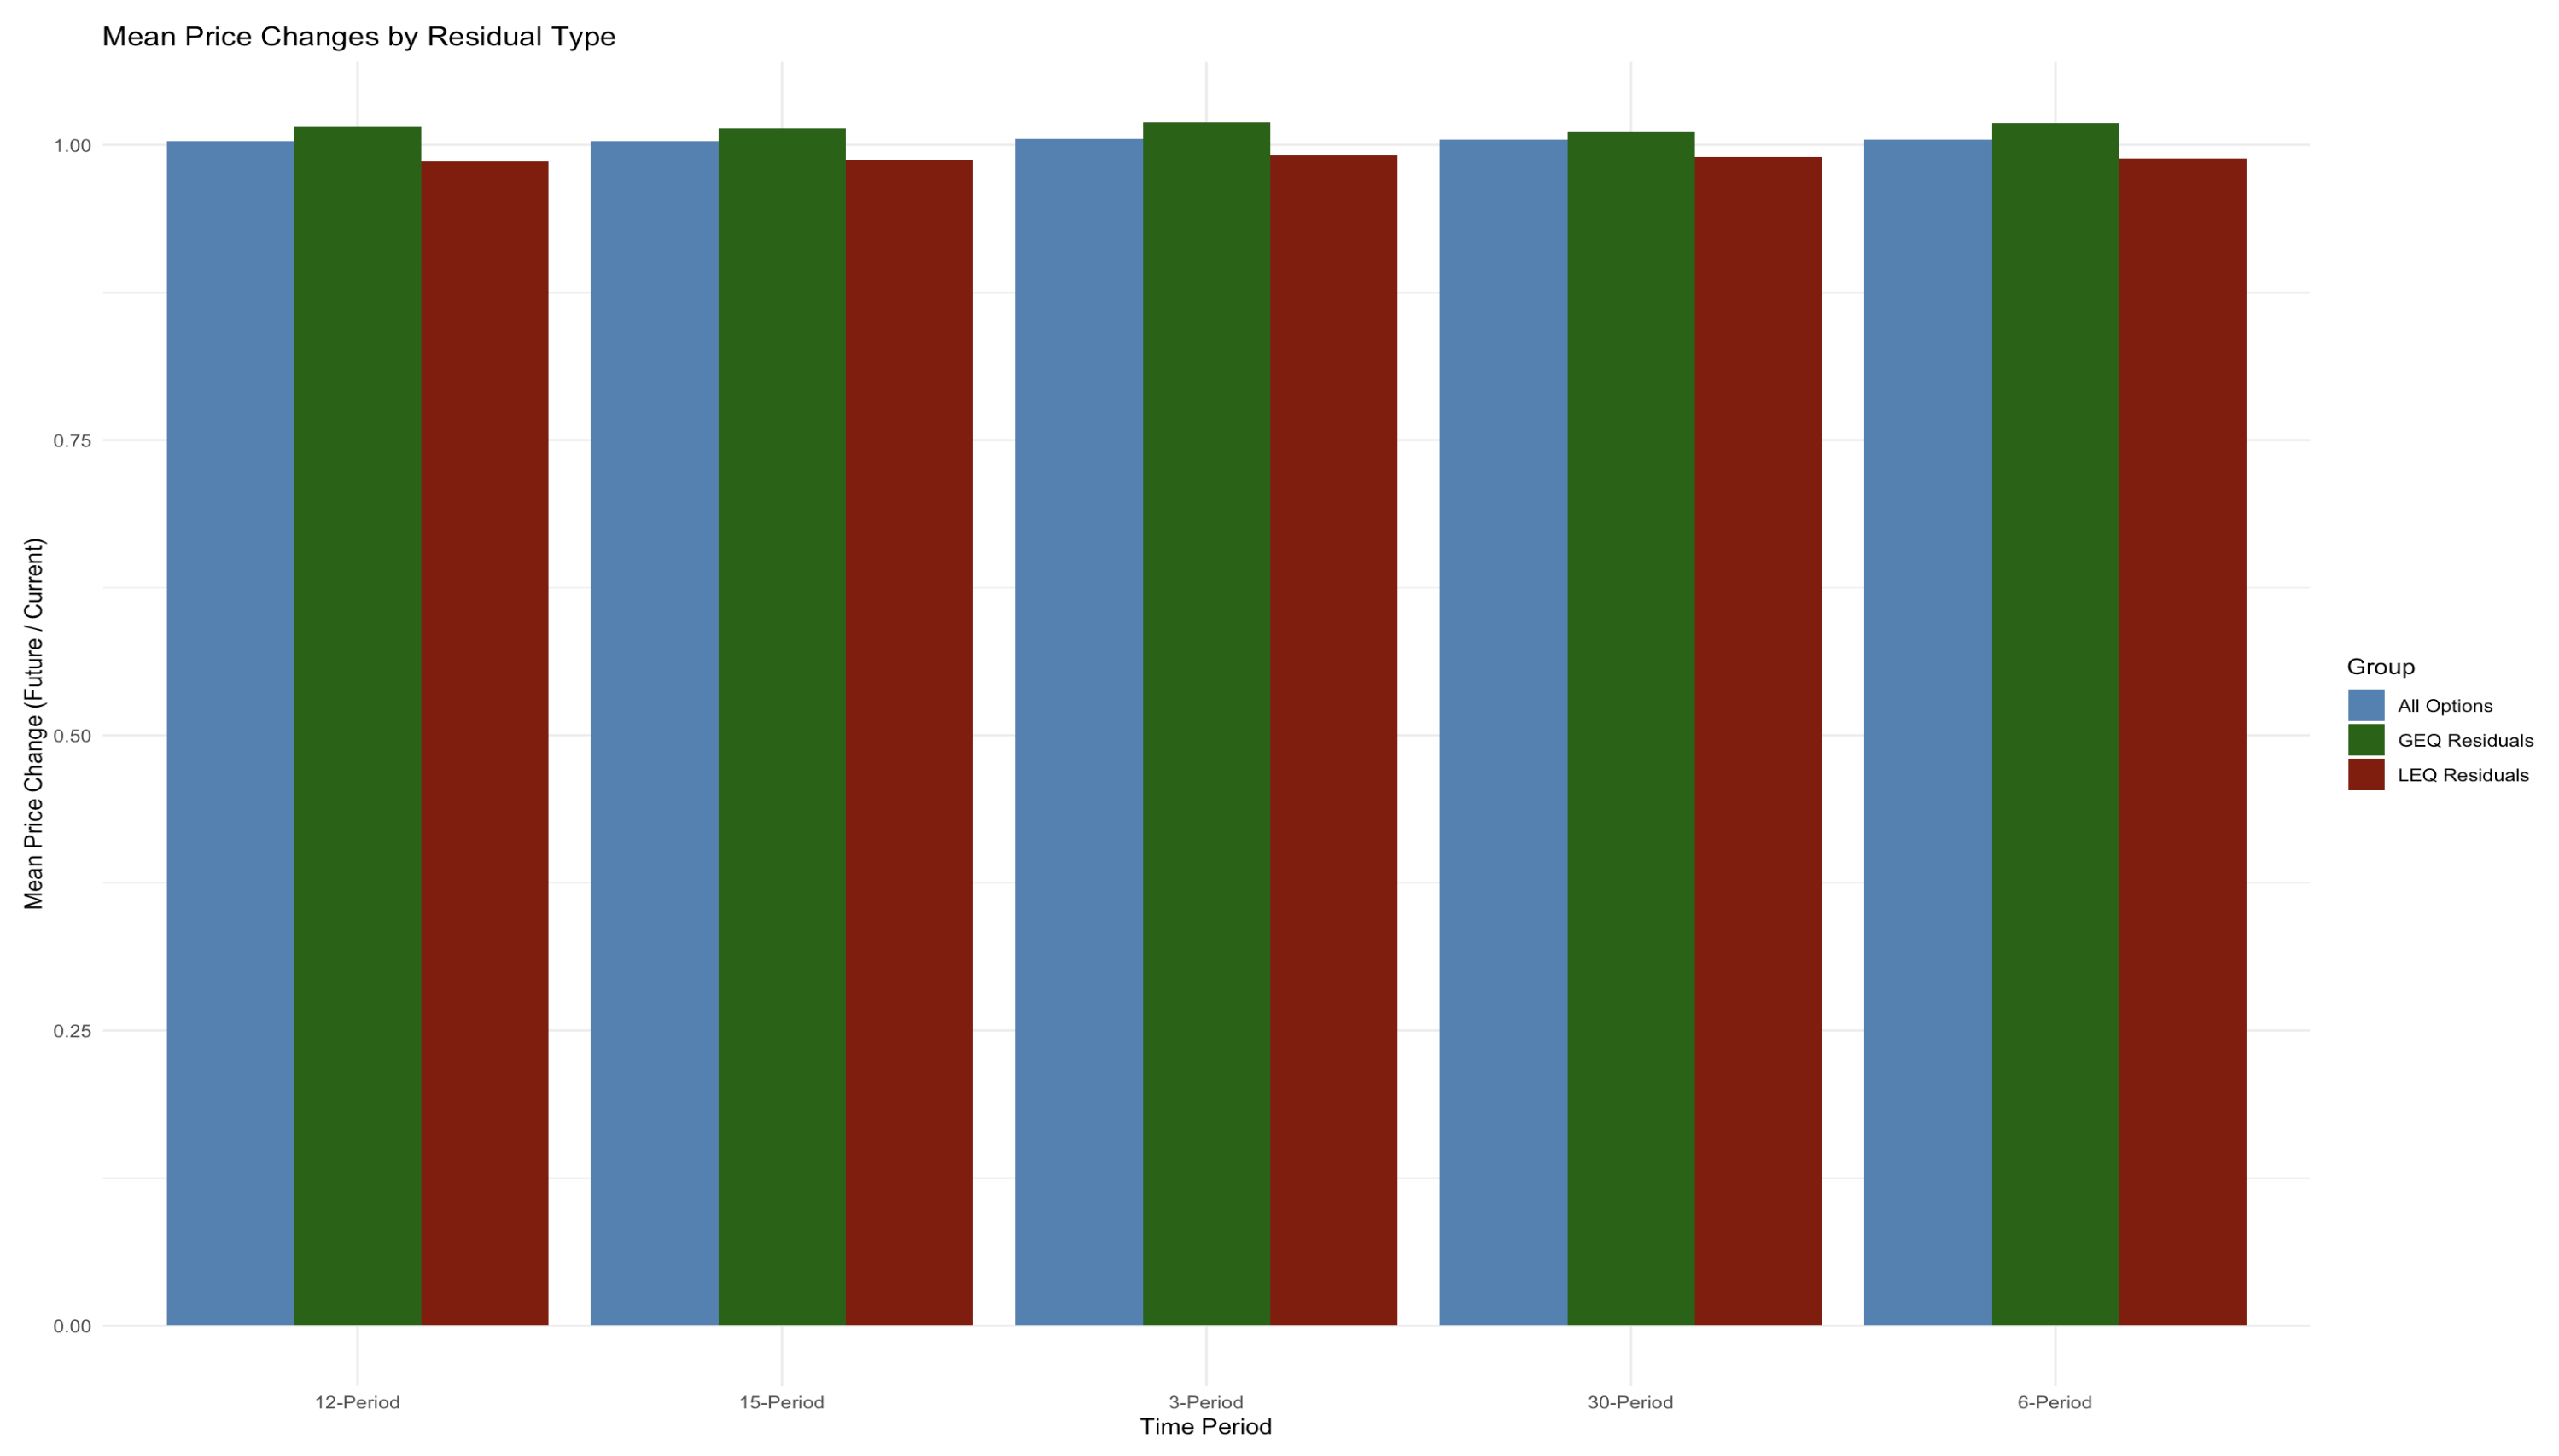
\includegraphics[width=0.8\linewidth]{data/results/mean_price_diff.png}
  \caption{Mean future price ratios by residual group}
  \label{fig:price-diff}
\end{figure}
\begin{table}[h]
  \centering
  \begin{tabular}{lcccccc}
    \toprule
    Period & GEQ & LEQ & Overall & $p_{\text{GEQ}}$ & $p_{\text{LEQ}}$ \\
    \midrule
    3  & 1.0111 & 0.9932 & 1.0019 & 0.0742 & 0     \\
    6  & 1.0125 & 0.9915 & 0.9991 & 0.0265 & 6e-04 \\
    12 & 1.0114 & 0.9889 & 0.9989 & 0.0504 & 3e-04 \\
    15 & 1.0086 & 0.9897 & 0.9975 & 0.0818 & 0.0052 \\
    30 & 1.0028 & 0.9889 & 0.9961 & 0.2437 & 0.0405 \\
    \bottomrule
  \end{tabular}
  \caption{Mean future price ratios by residual group with associated $p$-values.}
  \label{tab:mean-return}
\end{table}
\section{Discussion}
The KNN output served as a prior that highlighted relative mispricing. The residual-based signals produced consistent return differences in favor of positive residuals. While the profits observed in backtesting were modest, the approach performed better than random trading according to the null threshold. Further study could refine feature selection and risk controls.
\section{Conclusion}
The KNN model approximates $E(X\mid Y,Z,\ldots)$ and acts as a prior in a Bayesian decision rule. Trades are triggered when observed residuals cross the significance threshold. The strategy generated profits above a random baseline, suggesting predictive value in the modeled relationships.
\end{document}